\documentclass{article}

% Packages for formatting
\usepackage[margin=1in]{geometry}
\usepackage{fancyhdr}
\usepackage{enumitem}
\usepackage{graphicx}
\usepackage{kotex}
\usepackage{amsmath}
\usepackage{amsthm}
\usepackage{algorithm2e,setspace}
\usepackage{algpseudocode}
\usepackage{xcolor}
\usepackage{amssymb}

% Fonts
\usepackage[T1]{fontenc}
\usepackage[utf8]{inputenc}
\usepackage{newpxtext,newpxmath}
\usepackage{sectsty}

% Define colors
\definecolor{blue1}{HTML}{0077c2}
\definecolor{blue2}{HTML}{00a5e6}
\definecolor{blue3}{HTML}{b3e0ff}
\definecolor{blue4}{HTML}{00293c}
\definecolor{blue5}{HTML}{e6f7ff}

\definecolor{thmcolor}{RGB}{231, 76, 60}
\definecolor{defcolor}{RGB}{52, 152, 219}
\definecolor{lemcolor}{RGB}{155, 89, 182}
\definecolor{corcolor}{RGB}{46, 204, 113}
\definecolor{procolor}{RGB}{241, 196, 15}

\usepackage{color,soul}
\usepackage{soul}
\newcommand{\mathcolorbox}[2]{\colorbox{#1}{$\displaystyle #2$}}
\usepackage{cancel}
\newcommand\crossout[3][black]{\renewcommand\CancelColor{\color{#1}}\cancelto{#2}{#3}}
\newcommand\ncrossout[2][black]{\renewcommand\CancelColor{\color{#1}}\cancel{#2}}

\usepackage{hyperref}
\usepackage{booktabs}

% Chapter formatting
\definecolor{titleblue}{RGB}{0,53,128}
\usepackage{titlesec}
\titleformat{\section}
{\normalfont\sffamily\Large\bfseries\color{titleblue!100!gray}}{\thesection}{1em}{}
\titleformat{\subsection}
{\normalfont\sffamily\large\bfseries\color{titleblue!50!gray}}{\thesubsection}{1em}{}

%Tcolorbox
\usepackage[most]{tcolorbox}

%Tikzpicture
\usepackage{tikz-cd}
\usetikzlibrary{positioning}
\usetikzlibrary{angles, quotes}

% Header and footer formatting
\pagestyle{fancy}
\fancyhead{}
\fancyhf{}
\rhead{Student ID: 20192250\quad Name: 지용현}%\rule{3cm}{0.4pt}}
\lhead{\textcolor{blue2}{\textbf{CA Assignment \#1}}}
% Define footer
\newcommand{\footer}[1]{
	\begin{flushright}
		\vspace{2em}
		
\includegraphics[width=2cm]{school_logo.jpg} \\
		\vspace{1em}
		\textcolor{blue2}{\small\textbf{#1}}
	\end{flushright}
}
%\rfoot{\large Department of Information Security, Cryptogrphy and Mathematics, Kookmin Uni.
\includegraphics[height=1.5cm]{school_logo.jpg}}
\fancyfoot{}
\fancyfoot[C]{-\thepage-}

\newcommand{\ie}{\textnormal{i.e.}}
\newcommand{\rsa}{\mathsf{RSA}}
\newcommand{\rsacrt}{\mathsf{RSA}\textendash\mathsf{CRT}}
\newcommand{\inv}[1]{#1^{-1}}

\usepackage{amsthm}
\newtheorem{axiom}{Axiom}[section]
\newtheorem{theorem}{Theorem}
\newtheorem*{theorem*}{Theorem}
\newtheorem{proposition}[theorem]{Proposition}
\newtheorem{corollary}{Corollary}[theorem]
\newtheorem*{corollary*}{Corollary}
\newtheorem{lemma}[theorem]{Lemma}
\newtheorem*{lemma*}{Lemma}

\theoremstyle{definition}
\newtheorem{definition}{Definition}
\newtheorem*{definition*}{Definition}
\newtheorem{remark}{Remark}
\newtheorem{exercise}{Exercise}[section]

%New Command
\newcommand{\set}[1]{\left\{#1\right\}}
\newcommand{\N}{\mathbb{N}}
\newcommand{\Z}{\mathbb{Z}}
\newcommand{\Q}{\mathbb{Q}}
\newcommand{\R}{\mathbb{R}}
\newcommand{\C}{\mathbb{C}}
\newcommand{\F}{\mathbb{F}}
\newcommand{\nbhd}{\mathcal{N}}
\newcommand{\Log}{\operatorname{Log}}
\newcommand{\Arg}{\operatorname{Arg}}
\newcommand{\pv}{\operatorname{P.V.}}

\newcommand{\of}[1]{\left( #1 \right)} 
\newcommand{\abs}[1]{\left\lvert #1 \right\rvert}
\newcommand{\norm}[1]{\left\| #1 \right\|}

\newcommand{\sol}{\textcolor{magenta}{\bf Sol}}
\newcommand{\conjugate}[1]{\overline{#1}}


\renewcommand{\Re}{\operatorname{Re}}
\renewcommand{\Im}{\operatorname{Im}}

\begin{document}
	\pagenumbering{arabic}
	\begin{center}
		\huge\textbf{Complex Analysis}\\
		\vspace{0.5em}
	\end{center}
	
	\begin{enumerate}
		\item Show that the equation of a circle with center at $z_0$ and radius $R$ can be expressed by \[
		\abs{z}^2-2\Re\of{z\conjugate{z_0}}+\abs{z_0}^2=R^2.
		\]
		\begin{proof}[\sol]
			From the following figure: \begin{center}
				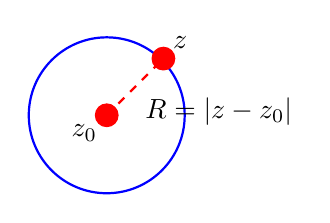
\begin{tikzpicture}[scale=1.8,>=Stealth]
				% draw axes
				%\draw[->, thick, black] (-2,0) -- (2,0) node[below right, black] {$\Re(z)$};
				%\draw[->, thick, black] (0,-2) -- (0,2) node[above left, black] {$\Im(z)$};
				
				% draw unit circle
				\draw[blue, thick] (0,0) circle (0.55cm) node[above left, black] {};
				
				% draw point
				\filldraw[red] (0,0) circle (0.08cm) node[below left, black] {$z_0$};
				\filldraw[red] (0.4,0.4) circle (0.08cm) node[anchor=south west, black] {$z$};
				
				% draw radius
				\draw[dashed, thick, red] (0,0) -- (0.4,0.4) node[midway, below right, black] {$R=\abs{z-z_0}$};
				
				% draw angle
				%\draw[->, thick, orange] (0.3,0) arc (0:45:0.3) node[midway, right, black] {$\theta$};
				\end{tikzpicture}
			\end{center} , a circle with center $z_0$ and radius $R$ can be represented as: $\abs{z-z_0}=R$. Then \begin{align*}
			\abs{z-z_0}=R &\implies \abs{z-z_0}^2=R^2\\
			&\implies\of{z-z_0}\of{\overline{z-z_0}}=R^2\quad\because\abs{z}^2=z\conjugate{z}\\
			&\implies z\conjugate{z}-z\conjugate{z_0}-z_0\conjugate{z}+z_0\conjugate{z_0}=R^2\\
			&\implies \abs{z}^2-(z\conjugate{z_0}+\conjugate{z}z_0)+\abs{z_0}^2=R^2\quad\because\abs{z}^2=z\conjugate{z}\\
			&\implies \abs{z}^2-2\Re(z\conjugate{z_0})+\abs{z_0}^2=R^2\quad\because\Re\of{z}=\frac{1}{2}\of{z+\conjugate{z}}.
			\end{align*}
		\end{proof}
		
		\item  Express all complex solutions to the equation $z^6 + 1 = 0$ in the form $z = a + bi$.
		\begin{proof}[\sol]
			For any complex number $z = r(\cos(\theta) + i\sin(\theta))$, the $n$-th roots are given by: \[
			z_k=\sqrt[n]{r}\left[\cos\of{\frac{\theta}{n}+\frac{2\pi}{n}\cdot k}+i\sin\of{\frac{\theta}{n}+\frac{2\pi}{n}\cdot k}\right],\quad k=0,1,2,\cdots,n-1.
			\] Let $n=6$, $r=1$, and $\theta = \pi$.
			\iffalse
			because \begin{center}
				\begin{center}
					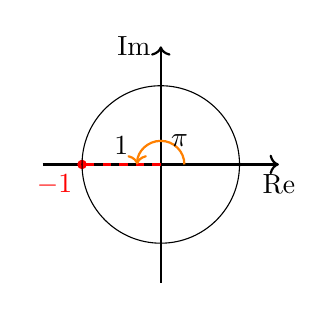
\begin{tikzpicture}
					\draw[thick,->] (-1.5,0) -- (1.5,0) node[below] {$\Re$};
					\draw[thick,->] (0,-1.5) -- (0,1.5) node[left] {$\Im$};
					
					% draw radius
					\draw[dashed, thick, red] (0,0) -- (-1,0) node[midway, above, black] {$1$};
					\draw[fill, red] (-1,0) circle (1.5pt) node[below left] {$-1$};
					\draw[->, thick, orange] (0.3,0) arc (0:180:0.3) node[midway, right, black] {$\pi$};
					\draw (0,0) circle (1);
					\end{tikzpicture}
				\end{center}
			\end{center}
			\fi
			Then \[
			z_k=\cos\of{\frac{\pi}{6}+\frac{\pi}{3}\cdot k}+i\sin\of{\frac{\pi}{6}+\frac{\pi}{3}\cdot k},\quad k=0,1,\cdots, 5.
			\]
			Note that: \begin{table}[ht!]
				\centering
				\begin{tabular}{c||c|c|c}
					\toprule
					Angle & $\sin(\theta)$ & $\cos(\theta)$ & $\tan(\theta)$ \\
					\midrule
					$0^\circ$ or $0$ & 0 & 1 & 0 \\
					$30^\circ$ or ${\pi}/{6}$ & ${1}/{2}$ & ${\sqrt{3}}/{2}$ & ${\sqrt{3}}/{6}$ \\
					$45^\circ$ or ${\pi}/{4}$ & ${1}/{\sqrt{2}}$ & ${1}/{\sqrt{2}}$ & 1 \\
					$60^\circ$ or ${\pi}/{3}$ & ${\sqrt{3}}/{2}$ & ${1}/{2}$ & $\sqrt{3}$ \\
					$90^\circ$ or ${\pi}/{2}$ & 1 & 0 & undefined \\
					$120^\circ$ or ${2\pi}/{3}$ & ${\sqrt{3}}/{2}$ & $-{1}/{2}$ & $-\sqrt{3}$ \\
					$135^\circ$ or ${3\pi}/{4}$ & ${1}/{\sqrt{2}}$ & $-{1}/{\sqrt{2}}$ & -1 \\
					$150^\circ$ or ${5\pi}/{6}$ & ${1}/{2}$ & $-{\sqrt{3}}/{2}$ & ${\sqrt{3}}/{3}$ \\
					$180^\circ$ or $\pi$ & 0 & -1 & 0 \\
					\bottomrule
				\end{tabular}
				%\caption{Special angles and their sine, cosine, and tangent values}
			\end{table}
			\newpage
			Computing the values for each $k$, we obtain the sixth roots of $-1$: \begin{itemize}
				\item[(i)] $k=0$: \[
				z_0=\cos\of{\frac{\pi}{6}}+i\sin\of{\frac{\pi}{6}}=\frac{\sqrt{3}}{2}+\frac{1}{2}i=\frac{1}{2}\of{\sqrt{3}+i}
				\]
				\item[(ii)] $k=1$: \[
				z_1=\cos\of{\frac{3\pi}{6}}+i\sin\of{\frac{3\pi}{6}}=0+i=i
				\]
				\item[(iii)] $k=2$: \[
				z_2=\cos\of{\frac{5\pi}{6}}+i\sin\of{\frac{5\pi}{6}}=-\frac{\sqrt{3}}{2}-\frac{1}{2}i=-\frac{1}{2}\of{\sqrt{3}+i}
				\]
				\item[(iv)] $k=3$: \[
				z_3=\cos\of{\frac{7\pi}{6}}+i\sin\of{\frac{7\pi}{6}}=-\frac{\sqrt{3}}{2}+\frac{1}{2}i=-\frac{1}{2}\of{\sqrt{3}-i}
				\]
				\item[(v)] $k=4$: \[
				z_4=\cos\of{\frac{9\pi}{6}}+i\sin\of{\frac{9\pi}{6}}=0-i=-i
				\]
				\item[(vi)] $k=5$: \[
				z_5=\cos\of{\frac{11\pi}{6}}+i\sin\of{\frac{11\pi}{6}}=\frac{\sqrt{3}}{2}-\frac{1}{2}i=\frac{1}{2}\of{\sqrt{3}-i}
				\]
			\end{itemize}
			Hence the complex solutions to the equation $z^6 + 1 = 0$ are:
			\begin{center}
				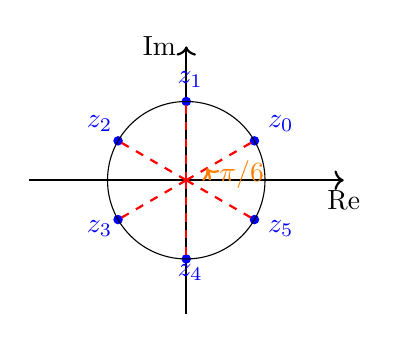
\begin{tikzpicture}
				\draw[thick,->] (-2.0,0) -- (2.0,0) node[below] {$\Re$};
				\draw[thick,->] (0,-1.7) -- (0,1.7) node[left] {$\Im$};
				
				\foreach \angle/\label [count=\k from 0] in {30/$z_0$, 90/$z_1$, 150/$z_2$, 210/$z_3$, 270/$z_4$, 330/$z_5$} {
					\coordinate (z\k) at (\angle:1);
					\draw[fill, blue] (z\k) circle (1.5pt) node[anchor={\angle-180}, shift={(0.05,0.05)}] {\label};
				}
				
				% draw radius
				\draw[dashed, thick, red] (0,0) -- (1.73/2,1/2) node[midway, above left, black] {};
				\draw[dashed, thick, red] (0,0) -- (0,1) node[midway, above left, black] {};
				\draw[dashed, thick, red] (0,0) -- (-1.73/2,-1/2) node[midway, above left, black] {};
				\draw[dashed, thick, red] (0,0) -- (-1.73/2,1/2) node[midway, above left, black] {};
				\draw[dashed, thick, red] (0,0) -- (0,-1) node[midway, above left, black] {};
				\draw[dashed, thick, red] (0,0) -- (1.73/2,-1/2) node[midway, above left, black] {};
				
				\draw[->, thick, orange] (0.3,0) arc (0:30:0.3) node[midway, right, orange] {$\pi/6$};
				\draw (0,0) circle (1);
				\end{tikzpicture}
			\end{center}
		\end{proof}
		
		\item Prove that, for any complex number $z = x + iy$, the following inequality holds: \[
		\abs{\exp\of{z^2}}\leq\exp\of{\abs{z}^2}.
		\]
		\begin{proof}[\sol]
			Let $z = x + iy$ be any complex number. We know that: \begin{align*}
			z^2 &= (x + iy)^2 = x^2 + 2ixy - y^2\ \text{and}\\
			|z|^2 &= z\bar{z} = (x + iy)(x - iy) = x^2 + y^2.
			\end{align*}
			
			We can rewrite the inequality as follows:
			\[
			\abs{\exp(x^2 + 2ixy - y^2)} \leq \exp(x^2 + y^2).
			\]
			Note that
			\[
			\abs{\exp(x^2 - y^2 + 2ixy)} = \exp(x^2 - y^2) \cdot \abs{\exp(2ixy)}=\exp\of{x^2-y^2}
			\] because:
			\[
			\abs{\exp(2ixy)} = \abs{\cos(2xy) + i\sin(2xy)} = \sqrt{\cos^2(2xy) + \sin^2(2xy)} = 1.
			\]
			
			So, we have:
			\[
			\exp(x^2 - y^2) \leq \exp(x^2 + y^2).
			\]
			
			Since the exponential function is strictly increasing, this inequality holds if and only if:
			\[
			x^2 - y^2 \leq x^2 + y^2,\quad\ie,\quad 0\leq 2y^2.
			\] This is true for all $y\in\R$. Therefore, the inequality $\abs{\exp(z^2)} \leq \exp(\abs{z}^2)$ holds for any complex number $z = x + iy$.
		\end{proof}
		
		\item A real-valued function $h(x, y)$ is said to be a \textit{harmonic function} if it satisfies the equation $h_{xx}+h_{yy}=0$. Let the function $f(z) = u(x, y) + i v(x, y)$ is a holomorphic function on a domain $D$. Prove that the functions $U(x, y)$ and $V(x, y)$ defined as follows: \[
		U(x,y)=e^{u(x,y)}\cos v\of{x,y},\quad V(x,y)=e^{u(x,y)}\sin v\of{x,y}
		\] are harmonic functions.
		\begin{proof}[\sol]
			Since $f(z)=u(x,y)+iv(x,y)$ is holomorphic, it satisfies the Cauchy-Riemann equations: \[
			u_x=v_y\quad\text{and}\quad u_y=-v_x
			\]
			Define a function $g(z) = \exp(f(z))$. Then $g(z)$ is also holomorphic, as it is the composition of the holomorphic functions $f(z)$ and $\exp(z)$. Note that
			\[
			g(z) = \exp\of{f\of{z}}=\exp(u(x, y) + iv(x, y)) = e^{u(x, y)}(\cos v(x, y) + i\sin v(x, y)).
			\]
			
			Observing the real and imaginary parts, we have \begin{align*}
			\Re\of{g(z)}&=e^{u\of{x,y}}\cos v\of{x,y} =: U(x,y)\quad \text{and}\\
			\Im\of{g(z)}&=e^{u\of{x,y}}\sin v\of{x,y} =: V(x,y).
			\end{align*} Since $g(z)$ is holomorphic, its real and imaginary parts satisfy the Cauchy-Riemann equations: \[
			U_x=V_y\quad\text{and}\quad U_y=-V_x.
			\]
			
			Then \begin{align*}
			U_{xx}&=\frac{\partial^2U}{\partial x^2}=\frac{\partial}{\partial x}\of{\frac{\partial U}{\partial x}}=\frac{\partial}{\partial x}\of{\frac{\partial V}{\partial y}}=\frac{\partial^2V}{\partial x\partial y}=\partial_{xy}V=V_{yx}\quad\text{and}\\
			U_{yy}&=\frac{\partial^2U}{\partial y^2}=\frac{\partial}{\partial y}\of{\frac{\partial U}{\partial y}}=\frac{\partial}{\partial y}\of{-\frac{\partial V}{\partial x}}=-\frac{\partial^2V}{\partial y\partial x}=-\partial_{yx}V=-V_{xy}.
			\end{align*}
			Since $U(x,y)$ and $V(x,y)$ are continuous, we have $V_{xy}=V_{yx}$ by Clairaut's theorem. Thus, \[
			U_{xx}+U_{yy}=V_{yx}+(-V_{xy})=0.
			\] That is, $U(x,y)$ is harmonic. By a similar argument, we can show that $V(x, y)$ is also harmonic.
		\end{proof}
		
		\newpage
		\item Show that, for trigonometric and hyperbolic functions defined on complex numbers, the following holds: \[
		\cosh z = \cosh x\cos y+i\sinh x\sin y
		\]  with $z=x+iy$ where $x,y\in\R$.
		\begin{proof}[\sol]
			Recall that \begin{align*}
			\cosh z= \cos\of{iz}=\frac{e^{z}+e^{-z}}{2}\quad\text{and}
			\quad\sinh z= \frac{1}{i}\sin\of{iz}=\frac{e^{z}-e^{-z}}{2}.
			\end{align*} Let $z=x+iy$. Then \begin{align*}
			\cosh z=\cosh\of{x+iy}&=\frac{e^xe^{iy}+e^{-x}e^{-iy}}{2}\\
			&=\frac{e^x\of{\cos y+i\sin y}+e^{-x}\of{\cos y-i\sin y}}{2}\\
			&=\frac{\of{e^x+e^{-x}}\cos y+i\of{e^x-e^{-x}}\sin y}{2}\\
			&=\cosh x\cos y+i\sinh x\sin y.
			\end{align*}
		\end{proof}
		
		\item The principal values of complex logarithm and complex exponential are defined as follows: for $z\neq 0$,
		\begin{align*}
		\Log\of{z} &:=\ln\abs{z}+i\Arg\of{z}\quad\text{and}\\
		\of{\pv}z^c &:=\exp\of{c\Log\of{z}}.
		\end{align*} Compute \begin{enumerate}
			\item $\Log\of{1-i}$ 
			\item $\of{\pv}\of{1+i}^i$
		\end{enumerate}
		\begin{proof}[\sol]
			\begin{enumerate}
				\item Recall that the complex logarithm can be defined as:
				\[\Log(z) = \ln|z| + i\Arg(z).
				\]
				Let $z = 1-i$ then the modulus is
				\[|1-i| = \sqrt{(1)^2 + (-1)^2} = \sqrt{2}.\]
				We can find the argument $\arg(1-i)$: \begin{align*}
				\tan(-\theta)=1\implies\theta=-\arctan\of{1}=-\frac{\pi}{4}.
				\end{align*}
				Now that we have the modulus and argument, we can compute the complex logarithm of $z = 1 - i$:
				\[
				\Log(1-i) = \ln|1-i| + i\Arg(1-i) = \ln\sqrt{2} - \frac{i\pi}{4}=\frac{1}{2}\ln 2+\frac{\pi}{4}i.
				\]
				\vspace{4pt}
				\item \begin{align*}
				\of{\pv}\of{1+i}^i &=\exp\of{i\Log\of{1+i}}\\
				&=\exp\of{i\of{\ln\abs{1+i}+i\Arg\of{1+i}}}\\
				&=\exp\of{i\of{\ln\sqrt{2}+\frac{i\pi}{4}}}\\
				&=e^{i\ln\sqrt{2}}e^{-\pi/4}\\
				&=\exp\of{-\frac{\pi}{4}}\of{\cos\of{\frac{\ln 2}{2}}+i\sin\of{\frac{\ln 2}{2}}}.
				\end{align*}
			\end{enumerate}
		\end{proof}
		
		\item Consider a complex function \[
		f\of{z}=\frac{z-\alpha}{1-\conjugate{\alpha}z}
		\] for $\abs{\alpha}<1$. Show that \begin{enumerate}
			\item $\abs{z}<1\implies\abs{f\of{z}}<1$ and
			\item $\abs{z}=1\implies\abs{f\of{z}}=1$.
		\end{enumerate}
		\begin{proof}[\sol]
			\begin{enumerate}
				\item Let $\abs{z}<1$. Consider $\abs{f\of{z}}^2$:
				\begin{align*}
				\left|\frac{z-a}{1-\conjugate{a}z}\right|^2=\frac{z-a}{1-\conjugate{a}z}\cdot\conjugate{\of{\frac{z-a}{1-\conjugate{a}z}}}&=\frac{z-a}{1-\conjugate{a}z}\cdot\frac{\conjugate{z}-\conjugate{a}}{1-a\conjugate{z}}\\
				&=\frac{z\conjugate{z}-a\conjugate{z}-\conjugate{a}z+a\conjugate{a}}{1-a\conjugate{z}-\conjugate{a}z+a\conjugate{a}z\conjugate{z}}\\
				&=\frac{\abs{z}^2-a\conjugate{z}-\conjugate{a}z+\abs{a}^2}{1-a\conjugate{z}-\conjugate{a}z+\abs{a}^2\abs{z}^2}\\
				&=\frac{\textcolor{red}{1}-a\conjugate{z}-\conjugate{a}z+\textcolor{red}{\abs{a}^2\abs{z}^2}+\abs{z}^2+\abs{a}^2\textcolor{blue}{-1}\textcolor{blue}{-\abs{a}^2\abs{z}^2}}{1-a\conjugate{z}-\conjugate{a}z+\abs{a}^2\abs{z}^2}\\
				&=1+\frac{\abs{z}^2+\abs{a}^2{-1}{-\abs{a}^2\abs{z}^2}}{(1-\conjugate{a}z)(1-a\conjugate{z})}\\
				&=1-\frac{{\abs{a}^2\abs{z}^2}-\abs{z}^2-\abs{a}^2+1}{\abs{1-\conjugate{a}z}^2}\\
				&=1-\frac{(1-\abs{z}^2)(1-\abs{a}^2)}{\abs{1-\conjugate{a}z}^2}\\
				&< 1-0\quad\because\abs{z}< 1, \abs{a}<1\\
				&=1.
				\end{align*} Thus \[
				\abs{f\of{z}}^2<1\implies\abs{f\of{z}}<1.
				\]
				
				\item Let $\abs{z}=1$ then \[
				\abs{f\of{z}}^2=1-\frac{(1-\abs{z}^2)(1-\abs{a}^2)}{\abs{1-\conjugate{a}z}^2}=1\implies\abs{f\of{z}}=1.
				\]
			\end{enumerate}
		\end{proof}
		
		\newpage
		\item Define a complex function as follows: \[
		f\of{z}=f\of{x+iy}=\begin{cases}
		\displaystyle\frac{3x^3-2y^3}{3x^2+2y^2}+i\frac{3x^3+2y^3}{3x^2+2y^2} &: z\neq 0\\
		0 &: z=0.
		\end{cases}
		\] \begin{enumerate}
			\item Does $f(z)$ satisfy the Cauchy-Riemann equation hold at $z=0$?
			\item Is $f(z)$ complex differentiable at $z=0$?
		\end{enumerate}
		\begin{proof}[\sol]
			\begin{enumerate}
				\item Let $f\of{z}=u(x,y)+iv(x,y)$ then \[
				u(x,y)=\begin{cases}\displaystyle
				\frac{3x^3-2y^3}{3x^2+2y^2}&: (x,y)\neq (0,0)\\
				0 &: (x,y)=(0,0)
				\end{cases},\quad
				v(x,y)=\begin{cases}\displaystyle
				\frac{3x^3+2y^3}{3x^2+2y^2} &: (x,y)\neq (0,0)\\
				0 &: (x,y)=(0,0).
				\end{cases}
				\] Note that \begin{align*}
				u_x(0,0)&=\lim\limits_{h\to 0}\frac{u(0+h,0)-u(0,0)}{h}=\lim\limits_{h\to 0}\frac{\frac{3h^3-0}{3h^2+0}-0}{h}=\lim\limits_{h\to 0}\frac{h}{h}=1,\\
				u_y(0,0)&=\lim\limits_{h\to 0}\frac{u(0,0+h)-u(0,0)}{h}=\lim\limits_{h\to 0}\frac{\frac{0-2h^3}{0+2h^2}-0}{h}=\lim\limits_{h\to 0}\frac{-h}{h}=-1,\\
				v_x(0,0)&=\lim\limits_{h\to 0}\frac{v(0+h,0)-v(0,0)}{h}=\lim\limits_{h\to 0}\frac{\frac{3h^3+0}{3h^2+0}-0}{h}=\lim\limits_{h\to 0}\frac{h}{h}=1,\\
				v_y(0,0)&=\lim\limits_{h\to 0}\frac{v(0,0+h)-v(0,0)}{h}=\lim\limits_{h\to 0}\frac{\frac{0+2h^3}{0+2h^2}-0}{h}=\lim\limits_{h\to 0}\frac{h}{h}=1.
				\end{align*}
				Thus $f$ satisfies CR-Eqs at $(0,0)$ since \[
				u_x(0,0)=1=v_y(0,0)\quad\text{and}\quad u_y(0,0)=-1=-v_x\of{0,0}.
				\]
				\vspace{4pt}
				\item Note that \[
				f'(0)=u_x(0,0)+iv_x(0,0)=1+i.
				\] However, for $\Delta z=\Delta t+i\Delta t=(1+i)\Delta t$, \begin{align*}
				 f'(0)=\lim\limits_{\Delta z\to 0}\frac{f\of{0+\Delta z}-f(0)}{\Delta z}&=\lim\limits_{\Delta t\to 0}\frac{f\of{1+\of{1+i}\Delta t}-f\of{0}}{\of{1+i}\Delta t}\\
				 &=\lim\limits_{\Delta t\to 0}\frac{\displaystyle\frac{3{\Delta t}^3-2{\Delta t}^3}{3{\Delta t}^2+2{\Delta t}^2}+i\frac{3{\Delta t}^3+2{\Delta t}^3}{3{\Delta t}^2+2{\Delta t}^2}}{\of{1+i}{\Delta t}}\\
				 &=\lim\limits_{\Delta t\to 0}\frac{1/5+i}{1+i}=\frac{3}{5}+\frac{2}{5}i\neq 1+i.
				\end{align*}
			\end{enumerate}
		\end{proof}
		
		\newpage
		\item The triangle $ABC$ is equilateral if the sides $a, b, c$ of $ABC$ satisfy the condition: \[
		a^2 + b^2 + c^2 - ab - bc - ca = 0.
		\]
		If a triangle with distinct complex numbers $\alpha,\beta$ and $\gamma$ as its vertices satisfies the equation \[
		\alpha^2+\beta^2+\gamma^2-\alpha\beta-\beta\gamma-\gamma\alpha=0,
		\] will it be an equilateral triangle?
		\begin{proof}[\sol]
			The complex solutions to the equation $z^3 + 1 = 0$ are:
			\begin{center}
				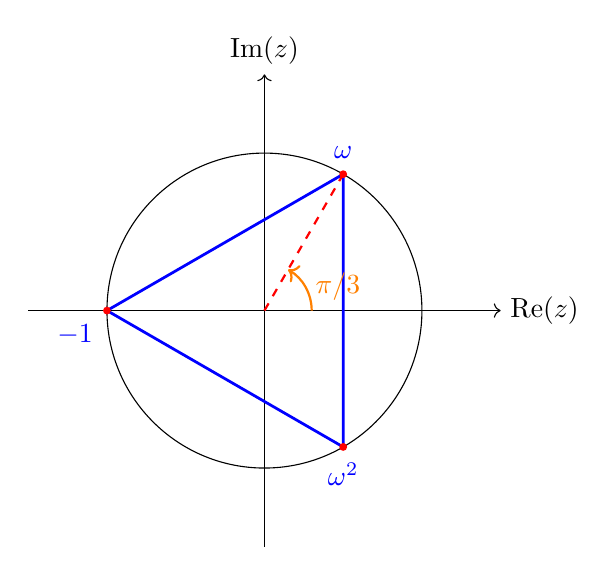
\begin{tikzpicture}[scale=2]
				
				% Draw the axes
				\draw[->] (-1.5, 0) -- (1.5, 0) node[right] {$\operatorname{Re}(z)$};
				\draw[->] (0, -1.5) -- (0, 1.5) node[above] {$\operatorname{Im}(z)$};
				
				% Draw the unit circle
				\draw (0, 0) circle (1);
				
				% Draw the solutions and connect them with a line
				\draw[blue, line width=1pt, rounded corners=1pt] (-1, 0) node[circle, fill=red, inner sep=1pt, label=below left:{$-1$}] {} -- (0.5, {sqrt(3)/2}) node[circle, fill=red, inner sep=1pt, label=above:{$\omega$}] {} -- (0.5, {-sqrt(3)/2}) node[circle, fill=red, inner sep=1pt, label=below:{$\omega^2$}] {} -- cycle;
				
				
				\draw[dashed, thick, red] (0,0) -- (1/2,{sqrt(3)/2}) node[midway, above left, black] {};
				
				\draw[->, thick, orange] (0.3,0) arc (0:60:0.3) node[midway, right, orange] {$\pi/3$};
				\end{tikzpicture}
		\end{center}
			Using $\omega^3-1=(\omega-1)\of{\omega^2+\omega+1}=0$, we have \begin{align*}
			\alpha^2+\beta^2+\gamma^2-\alpha\beta-\beta\gamma-\gamma\alpha&=(\textcolor{red}{\beta\gamma} - \gamma\alpha - \alpha\beta + \alpha^2) + (\beta^2\textcolor{blue}{-\beta\gamma} -\beta\gamma + \gamma^2)\\
			&=(\beta-\alpha)(\gamma-\alpha)+\of{\beta-\gamma}^2\\
			&=(\beta-\alpha)(\textcolor{red}{\beta}-\alpha\textcolor{blue}{-\beta}+\gamma)+\of{\beta-\gamma}^2\\
			&=(\beta-\alpha)^2\cdot 1+(\beta-\alpha)(\beta-\gamma)(-1)+\of{\beta-\gamma}^2\\
			&=(\beta-\alpha)^2\cdot\omega^3+(\beta-\alpha)(\beta-\gamma)\cdot(\omega^2+\omega)+\of{\beta-\gamma}^2\\
			&=\of{(\beta-\alpha)\omega+(\beta-\gamma)}\of{(\beta-\alpha)\omega^2+(\beta-\gamma)}\\
			&=0.
			\end{align*} Hence either $\of{\beta-\alpha}\omega=\gamma-\beta$ or $\of{\beta-\alpha}\omega^2=\gamma-\beta$. Note that \[
			\of{\beta-\alpha}\omega^2=\gamma-\beta\impliedby\of{\beta-\alpha}\omega^3=\of{\gamma-\beta}\omega\implies\beta-\alpha=\of{\gamma-\beta}\omega.
			\] Thus we have either \[
			\of{\beta-\alpha}\omega=\gamma-\beta\quad\text{or}\quad\beta-\alpha=\of{\gamma-\beta}\omega.
			\] That is, $\abs{\beta-\alpha}=\abs{\gamma-\beta}$, and the angle between the line segments joining $\alpha$to $\beta$ and $
			\alpha$ to $\gamma$ is $\pi/3$. Hence $\Delta\alpha\beta\gamma$ is equilateral.
		\end{proof}
	\end{enumerate}
	
	
	\footer{Department of Information Security, Cryptography and Mathematics, Kookmin University}
\end{document}
